\chapter{Backend Software}
------------------------

\section{Overview}
  In order to store and show the results sent from the {\bf FPGA} in a database a web server was developed; this server provides the user an interface where they can
see and manage the results, upload designs and configuration files to the {\bf chip tester} and administrate the database where the results have been stored. Basically
the web server ``serves'' the content to the user through the Internet to a web page, where the users (administrators or students) can check the results of their designs
or manage the results stored in the database. The users load their designs into the web server and then whenever the FPGA sends a ``download configuration files request''
to the server, it will send the files to the FPGA (if available).

\begin{figure}[htb]
\centering
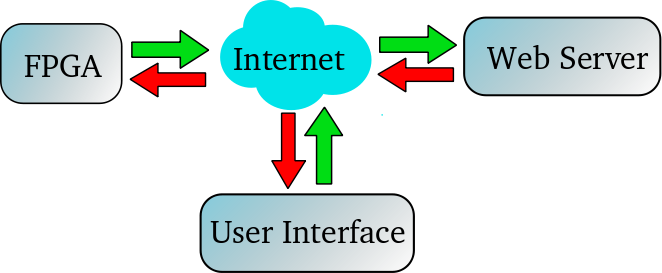
\includegraphics[scale = 0.4]{back_end_overview.png}
\caption{Interaction between elements in the system}
\label{fig:back_end_structure}
\end{figure}


 Nowadays almost every programming language provides libraries to develop web servers; for this application we required a robust, easy to use, programming language. Java, Python, PhP, Ruby,
Perl are the most common languages used to develop servers. We decided to use Ruby with its{\bf web framework} Sinatra. Ruby is a general-purpose object-oriented programming language easy to learn
and powerful, Sinatra is a Domain Specific Language (DSL) for quickly creating web applications in ruby.

UNICORN INSTEAD OF WEBBRICK, WHY?


\section{API}

The way the FPGA communicates to the server is through the Hypertext Transfer Protocol (HTTP). In the client-server model HTTP works as a request-response protocol. The FPGA and the user web browser act as clients, while the application running
on the computer hosting the web site is the server. The FPGA and web browser submit HTTP request messages to the server. The server stores content, provides resources such as configuration files, sends emails, manages the database on behalf of the clients.
HTTP defines 9 methods indicating the action to be performed on a resource: HEAD, GET, POST, PUT, DELETE, TRACE, OPTION, CONNECT and PATCH. To develop this application we have used only three of this methods {\bf GET} which retrieves information from the server,
{\bf POST} which sends data to the server as part of the request and {\bf DELETE} which deletes resources. The figure \ref{fig:get_example} shows an example of the get method, both in the server and in the browser.

\begin{figure}[htb]
\centering
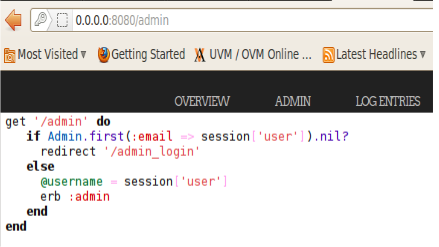
\includegraphics[scale = 0.6]{get.png}
\caption{Example of the HTTP method GET in the browser and in the server}
\label{fig:get_example}
\end{figure}

In order to communicate from the FPGA to the server a data exchange language is needed; the most popular data exchange language is ``XML'', nevertheless, adding the xml parsing libraries in the $\mu$Clinux
would slow down the parsing data process due to the complexity of the xml libraries. JSON, is a lightweight data exchange library supported in C (for the FPGA) and ruby (for the Server) therefore it was perfect
for our application. The figure \ref{fig:Json_message} shows an example of a message in the JSON format that would be sent from the FPGA to the server.

\begin{figure}[htb]
\centering
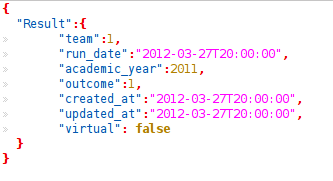
\includegraphics[scale = 0.6]{json_example.png}
\caption{Example of a JSON message}
\label{fig:Json_message}
\end{figure}

The table \ref{tab:api_server_fpga} shows the ``URL'' the FPGA uses to connect to the server, and a brief description of what each command does in the server.

\begin{table}
\centering
    \begin{tabular}{ | l | p{7.5cm} | p{5cm}|}
    \hline
    Type & Link & Command   \\ \hline
    post & /api/result & Stores the results sent from the fpga in the table Results in the database\\ \hline
    post & /api/result/:result\_id/design & Stores in the table Design\_Results associated to the result (in the table Results) identified with the id: result\_id (results summarized)\\ \hline
    post & /api/result/:result\_id/design/:design\_id	/measurement/frequency & Stores in the table FrequencyMeasurement associated to the design\_result identified with the id design\_id (information related to the frequency of the oscillator in the design)\\ \hline
    post & /api/result/:result\_id/design/:design\_id	/measurement/adc & Stores in the table AdcMeasurement associated to the design\_result identified with the id design\_id (information related to the sampled oscillator in the design)  \\ \hline
    post & /api/result/:result\_id/design/:design\_id	/vector & Stores in the table Test\_vector associated to the design\_result identified with the id design\_id (more information about the results of the test)\\ \hline
    get & /api/vdesign & Download a configuration file into the fpga\\ \hline
    \end{tabular}
    \caption{API for the communication between the fpga and the server}
    \label{tab:api_server_fpga}
\end{table}


\section{``Server'' (Sinatra stuff, database, etc)}

\begin{figure}[htb]
\centering
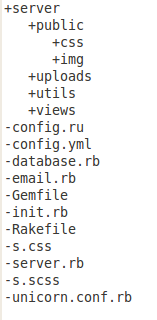
\includegraphics[scale = 0.5]{server_structure.png}
\caption{Folder structure of the server}
\label{fig:server_structure}
\end{figure}

  Inside the folder called {\bf server} are all the files regarding to our back-end application. In the folder {\bf public} are the stylesheets for the web page styling, and the images
displayed in the page, in {\bf uploads} are all the files uploaded in the server by the users, in {\bf utils} are some utility scripts written in ruby such as secure password generation,
{\bf views} contains all the views in the page that the different users can have access to.

\subsection{Database}

  Datamapper is an ORM (Object-Relational Mapping) that maps objects written in ruby to any supported database, thus giving freedom to the administrators of the system to use any database system (such as
MySQL, SQLite, Postgres,\ldots) to choose the database the administrator simply has to change the configuration parameters in the file {\bf config.yml} (found in the server folder) as shown in the
figure \ref{fig:database_config} where the administrator has set up the database system with MySql.

\begin{figure}[htb]
\centering
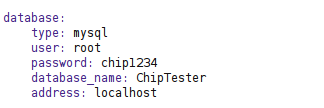
\includegraphics[scale = 0.6]{database_config.png}
\caption{Database system selection using the config.yml file}
\label{fig:database_config}
\end{figure}

In the table Admin \ref{tab:admin_table} is stored the administrators of the database. The email field is the email used t log in,
the Permission field is the level of authority that each administrator has. It can be either 0 or 1 (where 0 means that it can add
more administrators to the system) and the password\_hash field is a hash related to the user password (more in the server security section)
\begin{table}
\centering
    \begin{tabular}{ | l | l | l |}
    \hline
    Email & Permission & Password\_hash  \\ \hline
    String & Integer & BCryptHash \\ \hline
    \end{tabular}
    \caption{Admin table in the database}
    \label{tab:admin_table}
\end{table}

The initial administrator is configured in the archive config.yml as shown in the figure \ref{fig:admin_config}. For security reasons the password of
the initial administrator must be encrypted using the script {\bf pass.rb} located in server/utils. Whenever the server is run by the first time, or the database
has been created again this user will be mapped into the database, granting always access to the administrator.

\begin{figure}[htb]
\centering
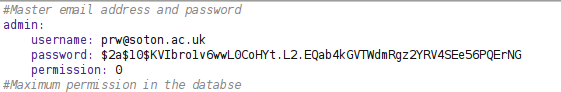
\includegraphics[scale = 0.75]{master_admin.png}
\caption{Initial Master Admin selection using the config.yml file}
\label{fig:admin_config}
\end{figure}

The File Upload table \ref{tab:file_upload_table} in the database stores the configuration files that has been uploaded to the server by the students.

\begin{table}
\centering
    \begin{tabular}{ | l | l | l | l | l | l | l |}
    \hline
    Id & Email & Team & File\_name & Is\_valid & Created\_at & Updated\_at  \\ \hline
    Serial & String & Integer & String & Boolean & Date & Date \\ \hline
    \end{tabular}
    \caption{File Upload table in the database}
    \label{tab:file_upload_table}
\end{table}

The Log entry table stores all the logs sent from the FPGA to the server, this table is displayed to the user in the web page.
\begin{table}
\centering
    \begin{tabular}{ | l | l | l | l | l | l | l |}
    \hline
    Id & Type & Message & File & Line & Created\_at & Updated\_at  \\ \hline
    Serial & Integer & String & String & Integer & Date & Date \\ \hline
    \end{tabular}
    \caption{Log Entry table in the database}
    \label{tab:log_entry_table}
\end{table}

The result table has
\begin{table}
\centering
    \begin{tabular}{ | l | l | l | l | l | l |}
    \hline
    Id & Team & Academic Year & Created\_at & Updated\_at & Virtual  \\ \hline
    Serial & Integer & String & Date & Date & Boolean \\ \hline
    \end{tabular}
    \caption{Result table in the database}
    \label{tab:Result_table}
\end{table}

\begin{table}
\centering
    \begin{tabular}{ | l | l | l | l | l | l | l |}
    \hline
    Id & Created\_at & Updated\_at & Triggers & File\_name & Clock\_Frequency & Design\_name  \\ \hline
    Id & Date & Date & String & String & String & String \\ \hline
    \end{tabular}
    \caption{Design Result table in the database}
    \label{tab:design_result_table}
\end{table}
\begin{center}

    \begin{tabular}{ | l | l | l | l | l | l | }
    \hline
    Id & Type & Input\_vector & Expected\_result & Actual\_result & Cycle\_count\\ \hline
    Serial & Integer & String & String & String & Integer \\ \hline
    \end{tabular}
\end{center}

\begin{table}
\centering
    \begin{tabular}{ | l | l | l | l | l |}
	\hline
       Trigger\_timeout & Has\_run & Fail & Created\_at & Updated\_at\\ \hline
       Boolean & Boolean & Boolean & Date & Date\\ \hline
    \end{tabular}
    \caption{Test Vector Result table in the database}
    \label{tab:Test_vector_result_table}
\end{table}

\begin{table}
\centering
    \begin{tabular}{| l | l | l | l |}
	\hline
       Id & Frequency & Created\_at & Updated\_at\\ \hline
       Serial & Float & Date & Date\\ \hline
    \end{tabular}
    \caption{Frequency Measurement table in the database}
    \label{tab:Frequency_measurement_table}
\end{table}

\subsection{Security}
BCRYPT
\subsection{Views}

\section{E-Mails}
Romel

\section{Remote Reconfiguration}
Romel

\section{User Interface}
% Pavlos

In order to provide an interface between the Superchip Tester, the database and the user, a webpage has been set up to provide the required functionality. The website provides access to the results database, but also allows the user to upload configuration files for the device.

The design of the webpage is based on a website template found on \href{http://www.freecsstemplates.org/}{CSS Templates}, altered to provide a look and functionality suitable for interface to the chip tester.

The webpage is laid out in a user-friendly and simple manner, with a navigation bar at the top of the page through which the user can browse the pages of the chip tester interface. The four entries in the navigation bar are \textit{Overview}, \textit{Admin}, \textit{Log Entries} and \textit{Upload Files}. In the main part of the screen, the content of the current view is displayed.

\begin{figure}[ht]
 \centering
 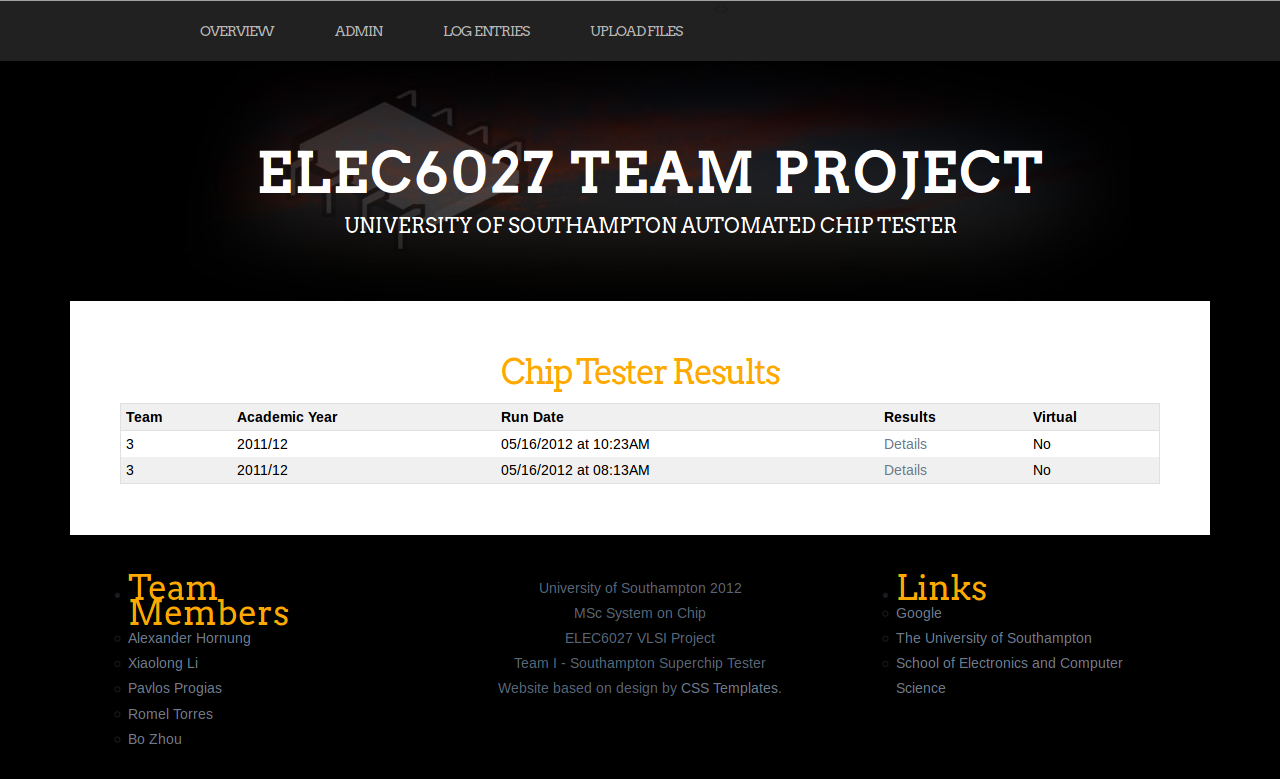
\includegraphics[width=0.95\textwidth]{web_if_overview}
 \caption{The ChipTester webpage showing an overview of the database.}
 \label{fig:web_if_overview}
\end{figure}

In figure \ref{fig:web_if_overview}, a screenshot of the website showing the first navigation option, \textit{Overview}. This view takes the user to an overview of the database where the superchip test results are stored. The table displays information on completed tests such as the number of the team, information regarding when the test was run and the relevant academic year and the result of the test.

Clicking on the result of an entry takes the user to a more detailed view of that specific run. In this view the user can also see the measured frequency of the oscillator of the design and the name of the design. If the design has failed the test, clicking on the failed result of the test takes the user to another view, where they can monitor the failed test in more detail. This page provides information on the failed test, to help identify the reason of the failure. In specific, the user can see information about the test run, including the input vector to the design and a comparison between the expected and the actual result.

The second option of the navigation bar, \textit{Admin} prompts the user to enter their administrator credentials and takes them to the administrator view page. From this page, an administrator can reset the database, e-mail the results to a specified e-mail address, go to a detailed view of the database or add a new administrator to the system.

\hl{more stuff about manage database}

Choosing the third option on the navigation bar, \textit{Log Entries}, \hl{take the user to yet another webpage that I can't explain what it does}.

The last option of the navigation bar, \textit{Upload Files} allows the user to upload a configuration file to the server. The user is asked to enter their e-mail and their team number and a file to upload.